\documentclass[mathserif,notheorems, hyperref={colorlinks, citecolor=blue, urlcolor=blue, linkcolor=blue}]{beamer}

\usepackage{amsmath}
\usepackage{amssymb}
\usepackage[scale=2]{ccicons}
\usepackage{appendixnumberbeamer}
\usepackage{booktabs}
\usepackage[toc,page]{appendix}
\usepackage{graphicx}
\usepackage{xspace}
\usepackage{adjustbox, lipsum}
\usepackage{bbm}
\usepackage{algorithm}
\usepackage{algpseudocode}
\usepackage[sort]{natbib}

% absolute positioning
\usepackage[absolute,overlay]{textpos}

%% source for images.
\newcommand{\source}[1]{{\let\thefootnote\relax\footnote{{\tiny #1}}}}

\pdfstringdefDisableCommands{%
  \def\\{}%
  \def\texttt#1{<#1>}%
}

\makeatletter
\let\save@measuring@true\measuring@true
\def\measuring@true{%
  \save@measuring@true
  \def\beamer@sortzero##1{\beamer@ifnextcharospec{\beamer@sortzeroread{##1}}{}}%
  \def\beamer@sortzeroread##1<##2>{}%
  \def\beamer@finalnospec{}%
}
\makeatother

\input{macros/math}
\usepackage{simplebeam}

%% tikz

\usepackage{tikz}
\usepackage{pgfplots}
\usepgfplotslibrary{fillbetween}
\usetikzlibrary{patterns}
%% pgf and tikz options.
\pgfplotsset{
    compat=1.5.1,
    oracle/.style={color=red, style=dashed, line width=1.5pt},
    bound/.style={color=blue, style=solid, line width=1.5pt},
    objective/.style={color=black, style=solid, line width=1.5pt},
}

\tikzset{
    font={\fontsize{18pt}{12}\selectfont},
}


\title{}
\author{}
\institute{}
\date{}


\begin{document}
    %% TODO: Should write custom title template instead of this slide.
    \setbeamercolor{background canvas}{bg=lightcyan}
        \begin{frame}
        \vspace{1em}
        \begin{center}
            {\Large Interpolation, Growth Conditions, and Stochastic Gradient Descent  \vspace{1em}} %% title

            {\large Aaron Mishkin, \\ \texttt{amishkin@cs.ubc.ca} } %% author
        \end{center}

        \vspace{1ex}

       \begin{figure}
            \centering
            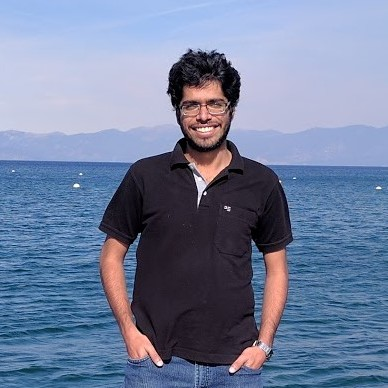
\includegraphics[width=0.18\textwidth]{collaborators/sharan}
            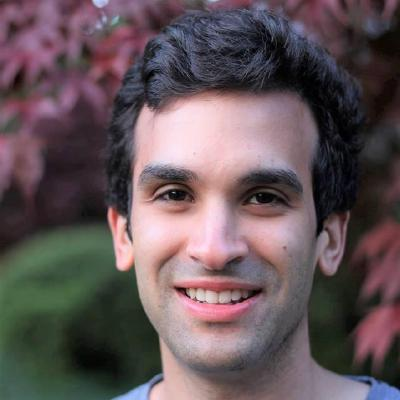
\includegraphics[width=0.18\textwidth]{collaborators/issam}
            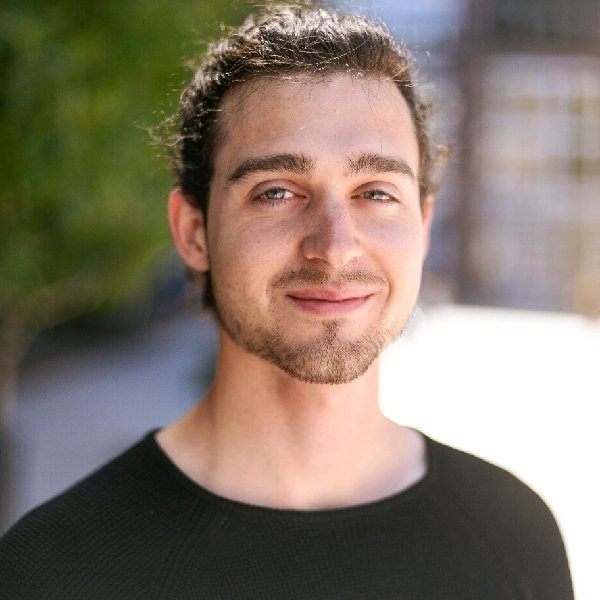
\includegraphics[width=0.18\textwidth]{collaborators/gauthier}
            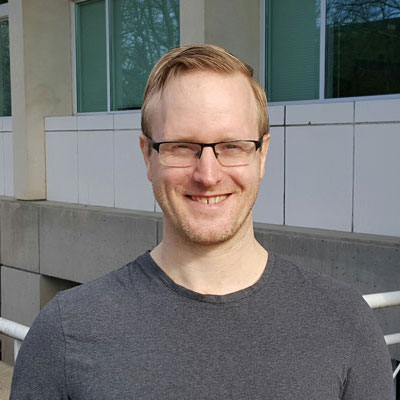
\includegraphics[width=0.18\textwidth]{collaborators/mark}
            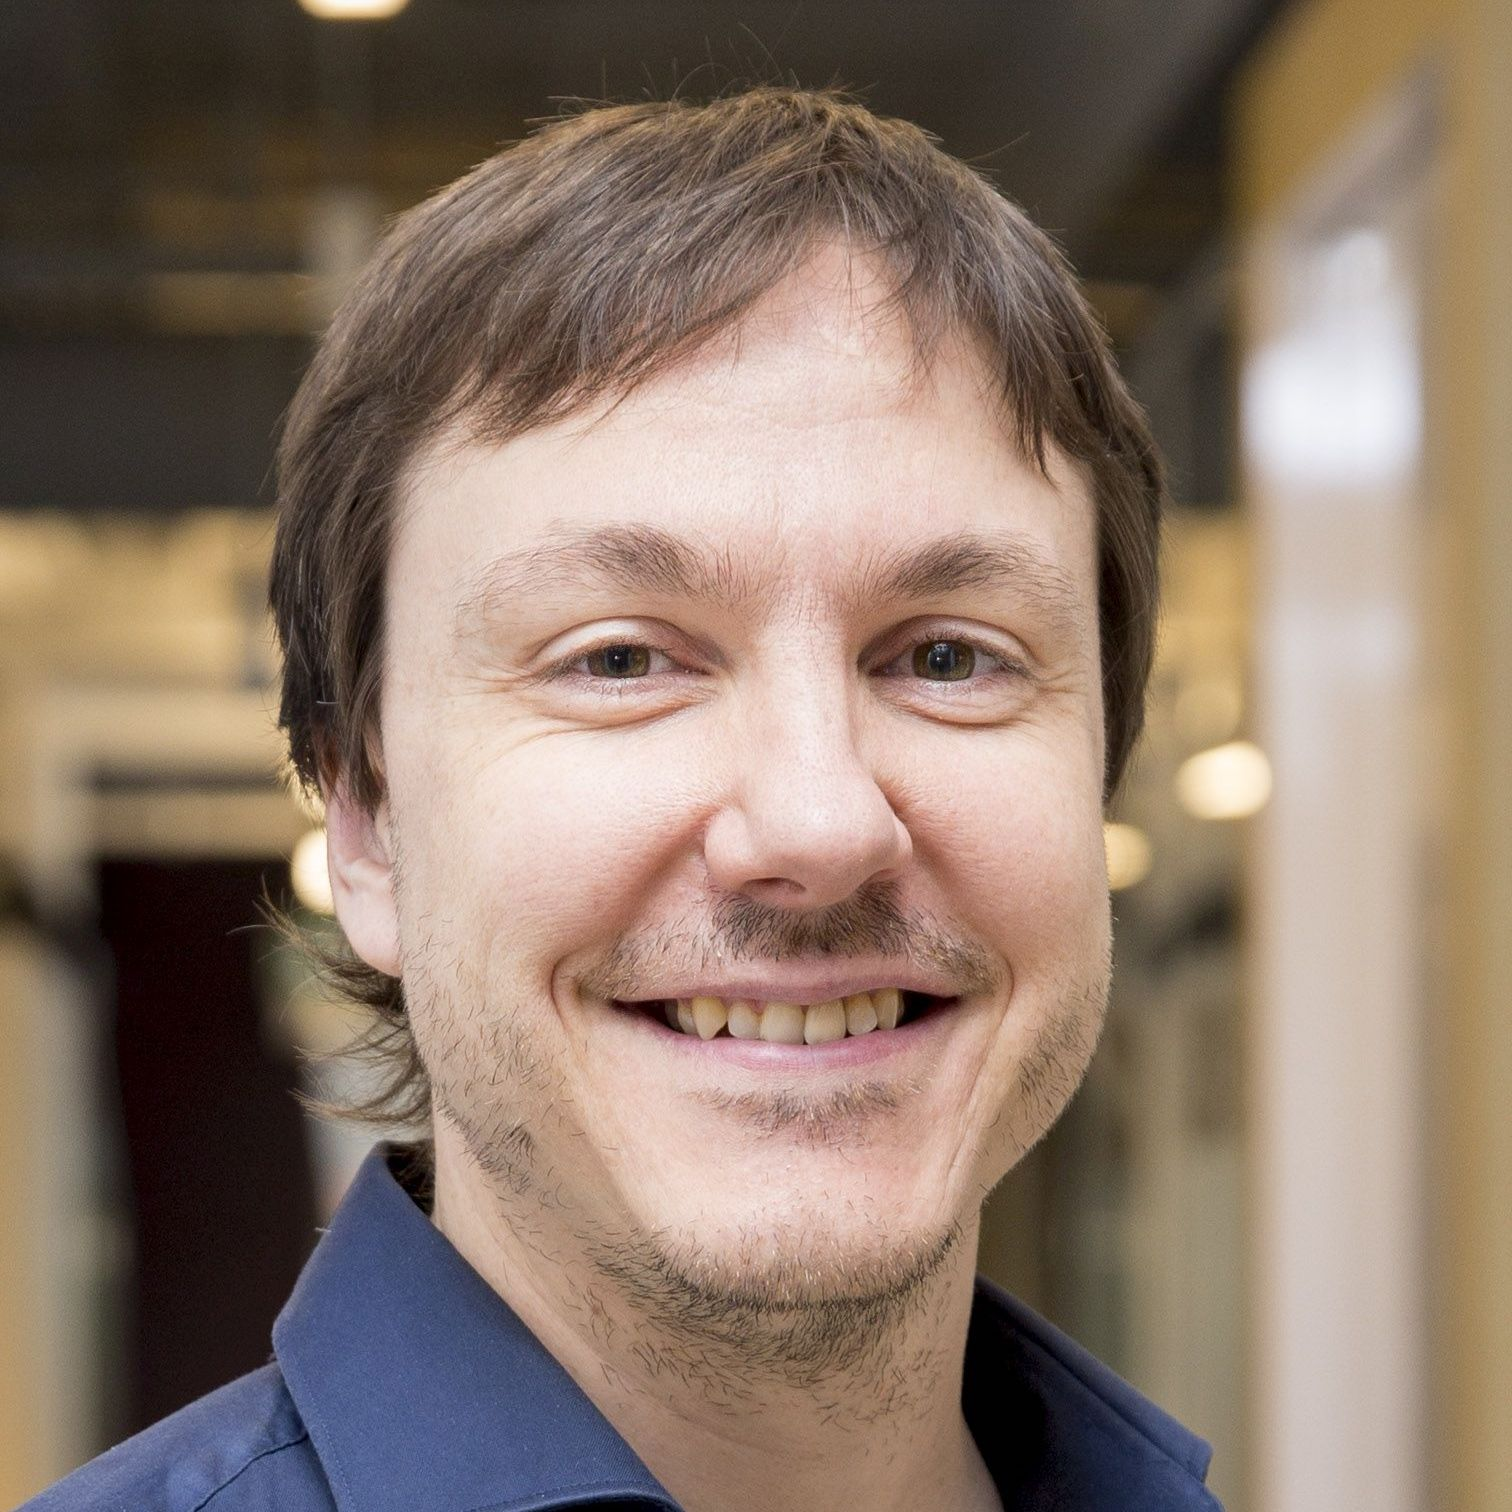
\includegraphics[width=0.18\textwidth]{collaborators/simon}

            \vspace{0.4ex}%

            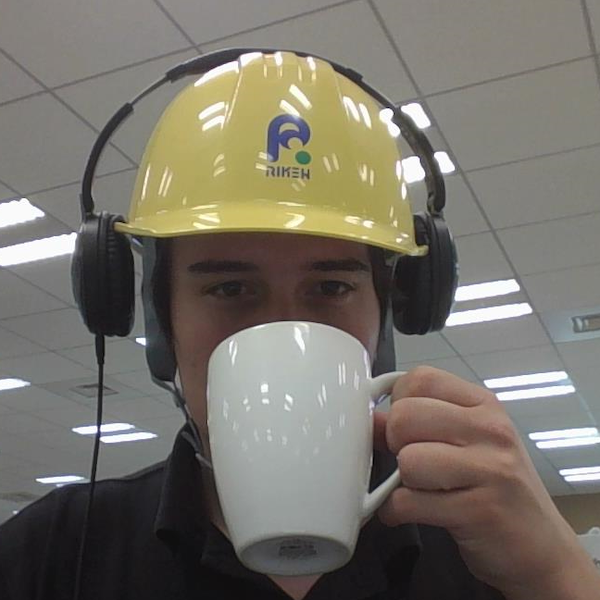
\includegraphics[width=0.18\textwidth]{collaborators/fred}
            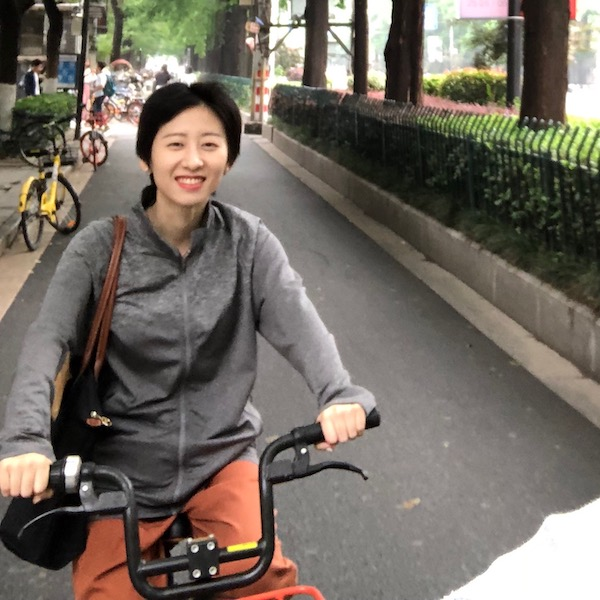
\includegraphics[width=0.18\textwidth]{collaborators/cathy}
            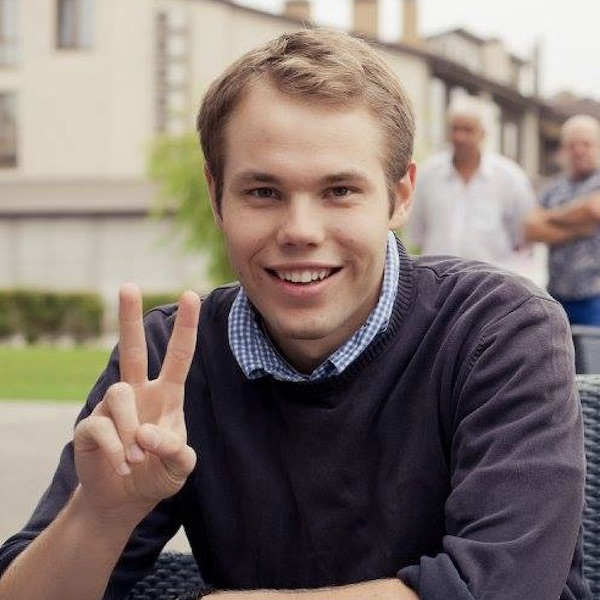
\includegraphics[width=0.18\textwidth]{collaborators/wilder}
            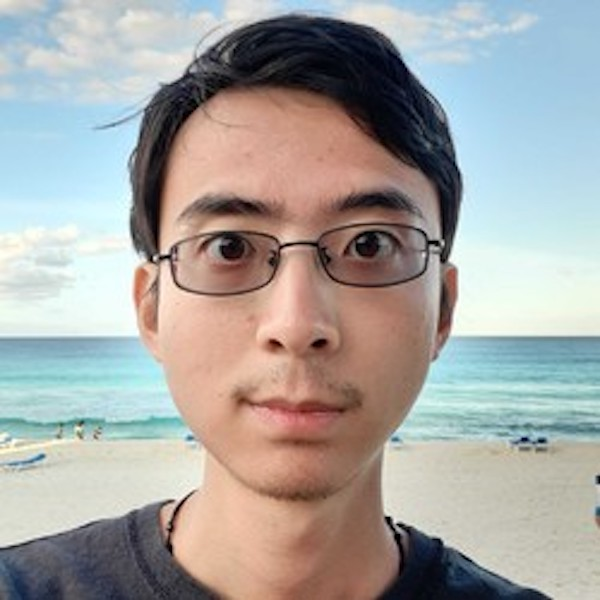
\includegraphics[width=0.18\textwidth]{collaborators/joey}
        \end{figure}
    \end{frame}
   
    \setbeamercolor{background canvas}{bg=white}
  
    \begin{frame}{Training neural networks is dangerous work!}
       
       \begin{figure}
            \centering
            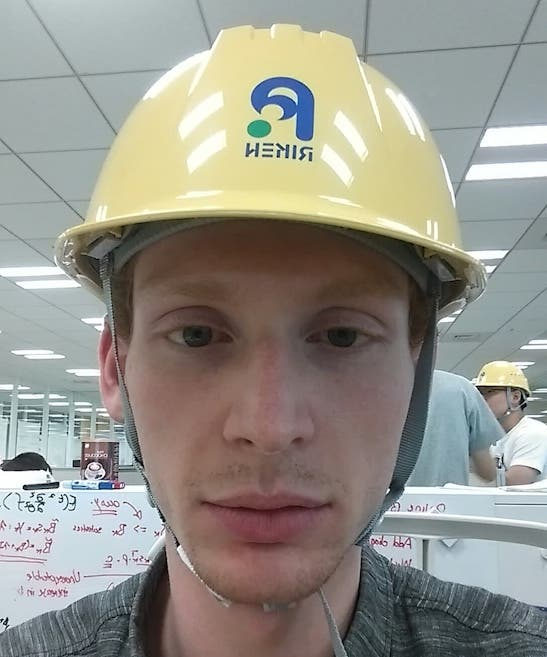
\includegraphics[width=0.45\textwidth]{collaborators/helmet1} 
            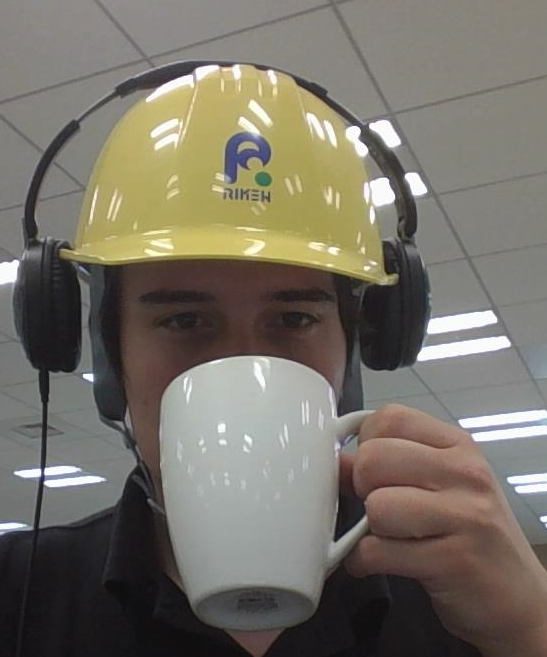
\includegraphics[width=0.45\textwidth]{collaborators/helmet2} 
       \end{figure} 
    \end{frame}
   
    \begin{frame}{Goal}
        \Large 
        
        \textbf{Premise}: modern neural networks are extremely flexible and can exactly fit current training datasets. 
       
        \vspace{1ex} 

        \textbf{Question}: what is the complexity of learning such models using stochastic gradient descent (SGD)?% 
        
        \vspace{1ex} 
        \pause%
        \rule{\textwidth}{0.4pt}% 
        \vspace{1ex} 

        \textbf{Main Works}:
        \begin{itemize}
            \item \citet*{schmidt2013fast}
            \item \citet*{vaswani2019fast}
            \item \citet*{vaswani2019painless}
        \end{itemize}

    \end{frame}

    \begin{frame}{Talk Roadmap}
        \textbf{Part 1: Interpolation}
        \begin{itemize}
            \item Assumptions and oracle model of stochastic optimization.
            \item Formal definitions of interpolation.
        \end{itemize}

        \vspace{2ex}
        
        \textbf{Part 2: Growth Conditions}
        \begin{itemize}
            \item The strong and weak growth conditions. 
            \item Connections between interpolation and strong/weak growth.
        \end{itemize}
        
        \vspace{2ex}

        \textbf{Part 3: First-Order Methods under Interpolation}
        \begin{itemize}
            \item SGD with a fixed step-size.
            \item Parameter-free SGD using an Armijo line-search.
            \item Accelerating stochastic gradient descent. 
        \end{itemize}
    \end{frame}

    \begin{frame}{Motivation: Model Fitting in ML}
       
       \begin{figure}
            \centering
            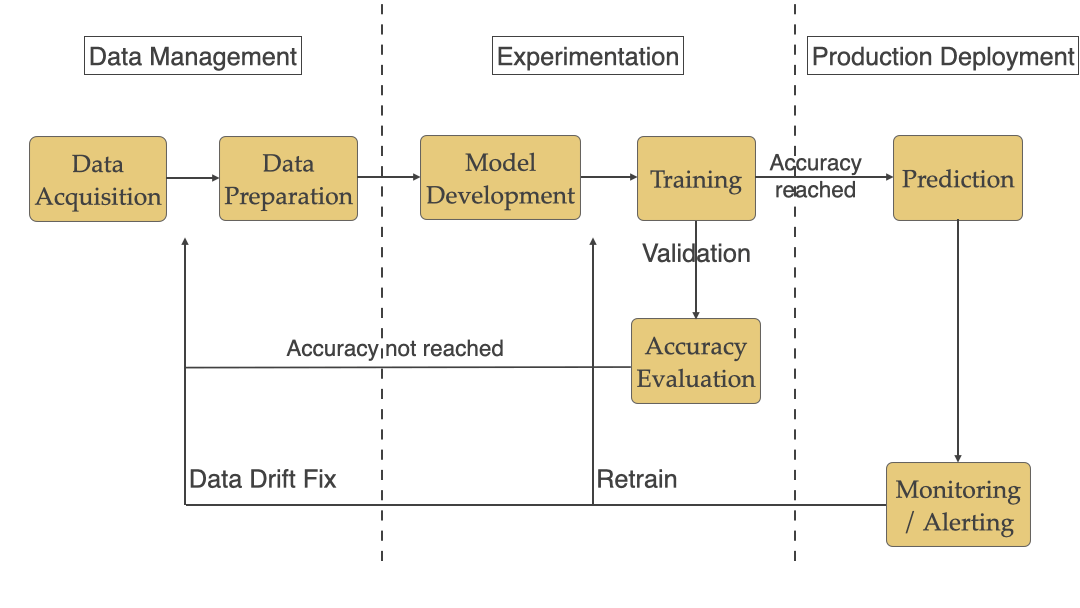
\includegraphics[width=0.98\textwidth]{figures/workflow} 
       \end{figure} 

       \source{https://towardsdatascience.com/challenges-deploying-machine-learning-models-to-production-ded3f9009cb3}
    \end{frame}

    \begin{frame}{Motivation: Model Fitting in ML}
       
       \begin{figure}
            \centering
            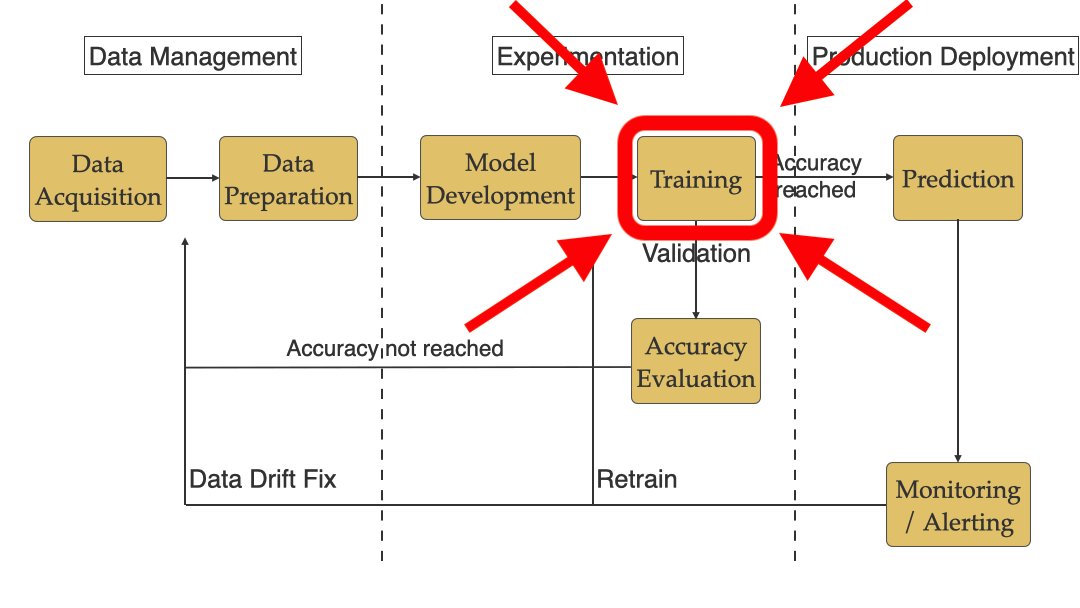
\includegraphics[width=0.98\textwidth]{figures/workflow_highlighted} 
       \end{figure} 

       \source{https://towardsdatascience.com/challenges-deploying-machine-learning-models-to-production-ded3f9009cb3}
    \end{frame}
    
    \begin{frame}{Motivation: Stochastic Gradient Descent}

        \begin{center}
            \Large
            ``Stochastic gradient descent (SGD) is today one of the main workhorses for solving large-scale supervised learning and optimization problems.''\\
            ---\citet{drori2019complexity}
        \end{center}

    \end{frame}

    \begin{frame}{Motivation: Consensus Says\ldots}

        \begin{center}
            \Large \dots and also~\citet{xu2017second,
            zhang2016parallel,
            patterson2017deep,
            pillaud2018statistical,
            grosse2015scaling,
            assran2018stochastic,
            damaskinos2019aggregathor,
            kawaguchi2020ordered,
            bernstein2018signsgd,
            li2019rsa,
            agarwal2017second,
            hofmann2015variance,
            geffner2019rule,
            assran2020convergence,
            gower2019sgd}
        \end{center}

    \end{frame}

    \begin{frame}{Motivation: Challenges in Optimization for ML}

        \textbf{Stochastic gradient methods} are the most popular algorithms for fitting ML models,
        \begin{align*}
            \textbf{SGD:} \quad w_{k + 1} = w_k - \eta_k \nabla f_i \, (w_k). \\
        \end{align*}

        % SGD is scalable and converges if $\eta_k$ decreases sufficiently slowly.\vspace{1em}

        But practitioners face major challenges with \vspace{0.5em}
        \begin{itemize}
            \item \textbf{Speed}: step-size/averaging controls convergence rate.
            \item \textbf{Stability}: hyper-parameters must be tuned carefully.
            \item \textbf{Generalization}: optimizers encode statistical tradeoffs.
        \end{itemize}
        \vspace{1em}

    \end{frame}


    \begin{frame}{Motivation: Challenges in Optimization for ML}

        \textbf{Stochastic gradient methods} are the most popular algorithms for fitting ML models,
        \begin{align*}
            \textbf{SGD:} \quad w_{k + 1} = w_k - \eta_k \nabla f_i \, (w_k). \\
        \end{align*}

        % SGD is scalable and converges if $\eta_k$ decreases sufficiently slowly.\vspace{1em}

        But practitioners face major challenges with \vspace{0.5em}
        \begin{itemize}
            \item \textcolor{red}{\textbf{Speed}: step-size/averaging controls convergence rate.}
            \item \textcolor{red}{\textbf{Stability}: hyper-parameters must be tuned carefully.}
            \item \textbf{Generalization}: optimizers encode statistical tradeoffs.
        \end{itemize}
        \vspace{1em}

    \end{frame}

    \begin{frame}{Motivation: Trends on CIFAR-10} 
        \begin{center}
            \Large Test Accuracy: \textbf{CIFAR-10}
        \end{center}

        \begin{figure}[]
            \centering
            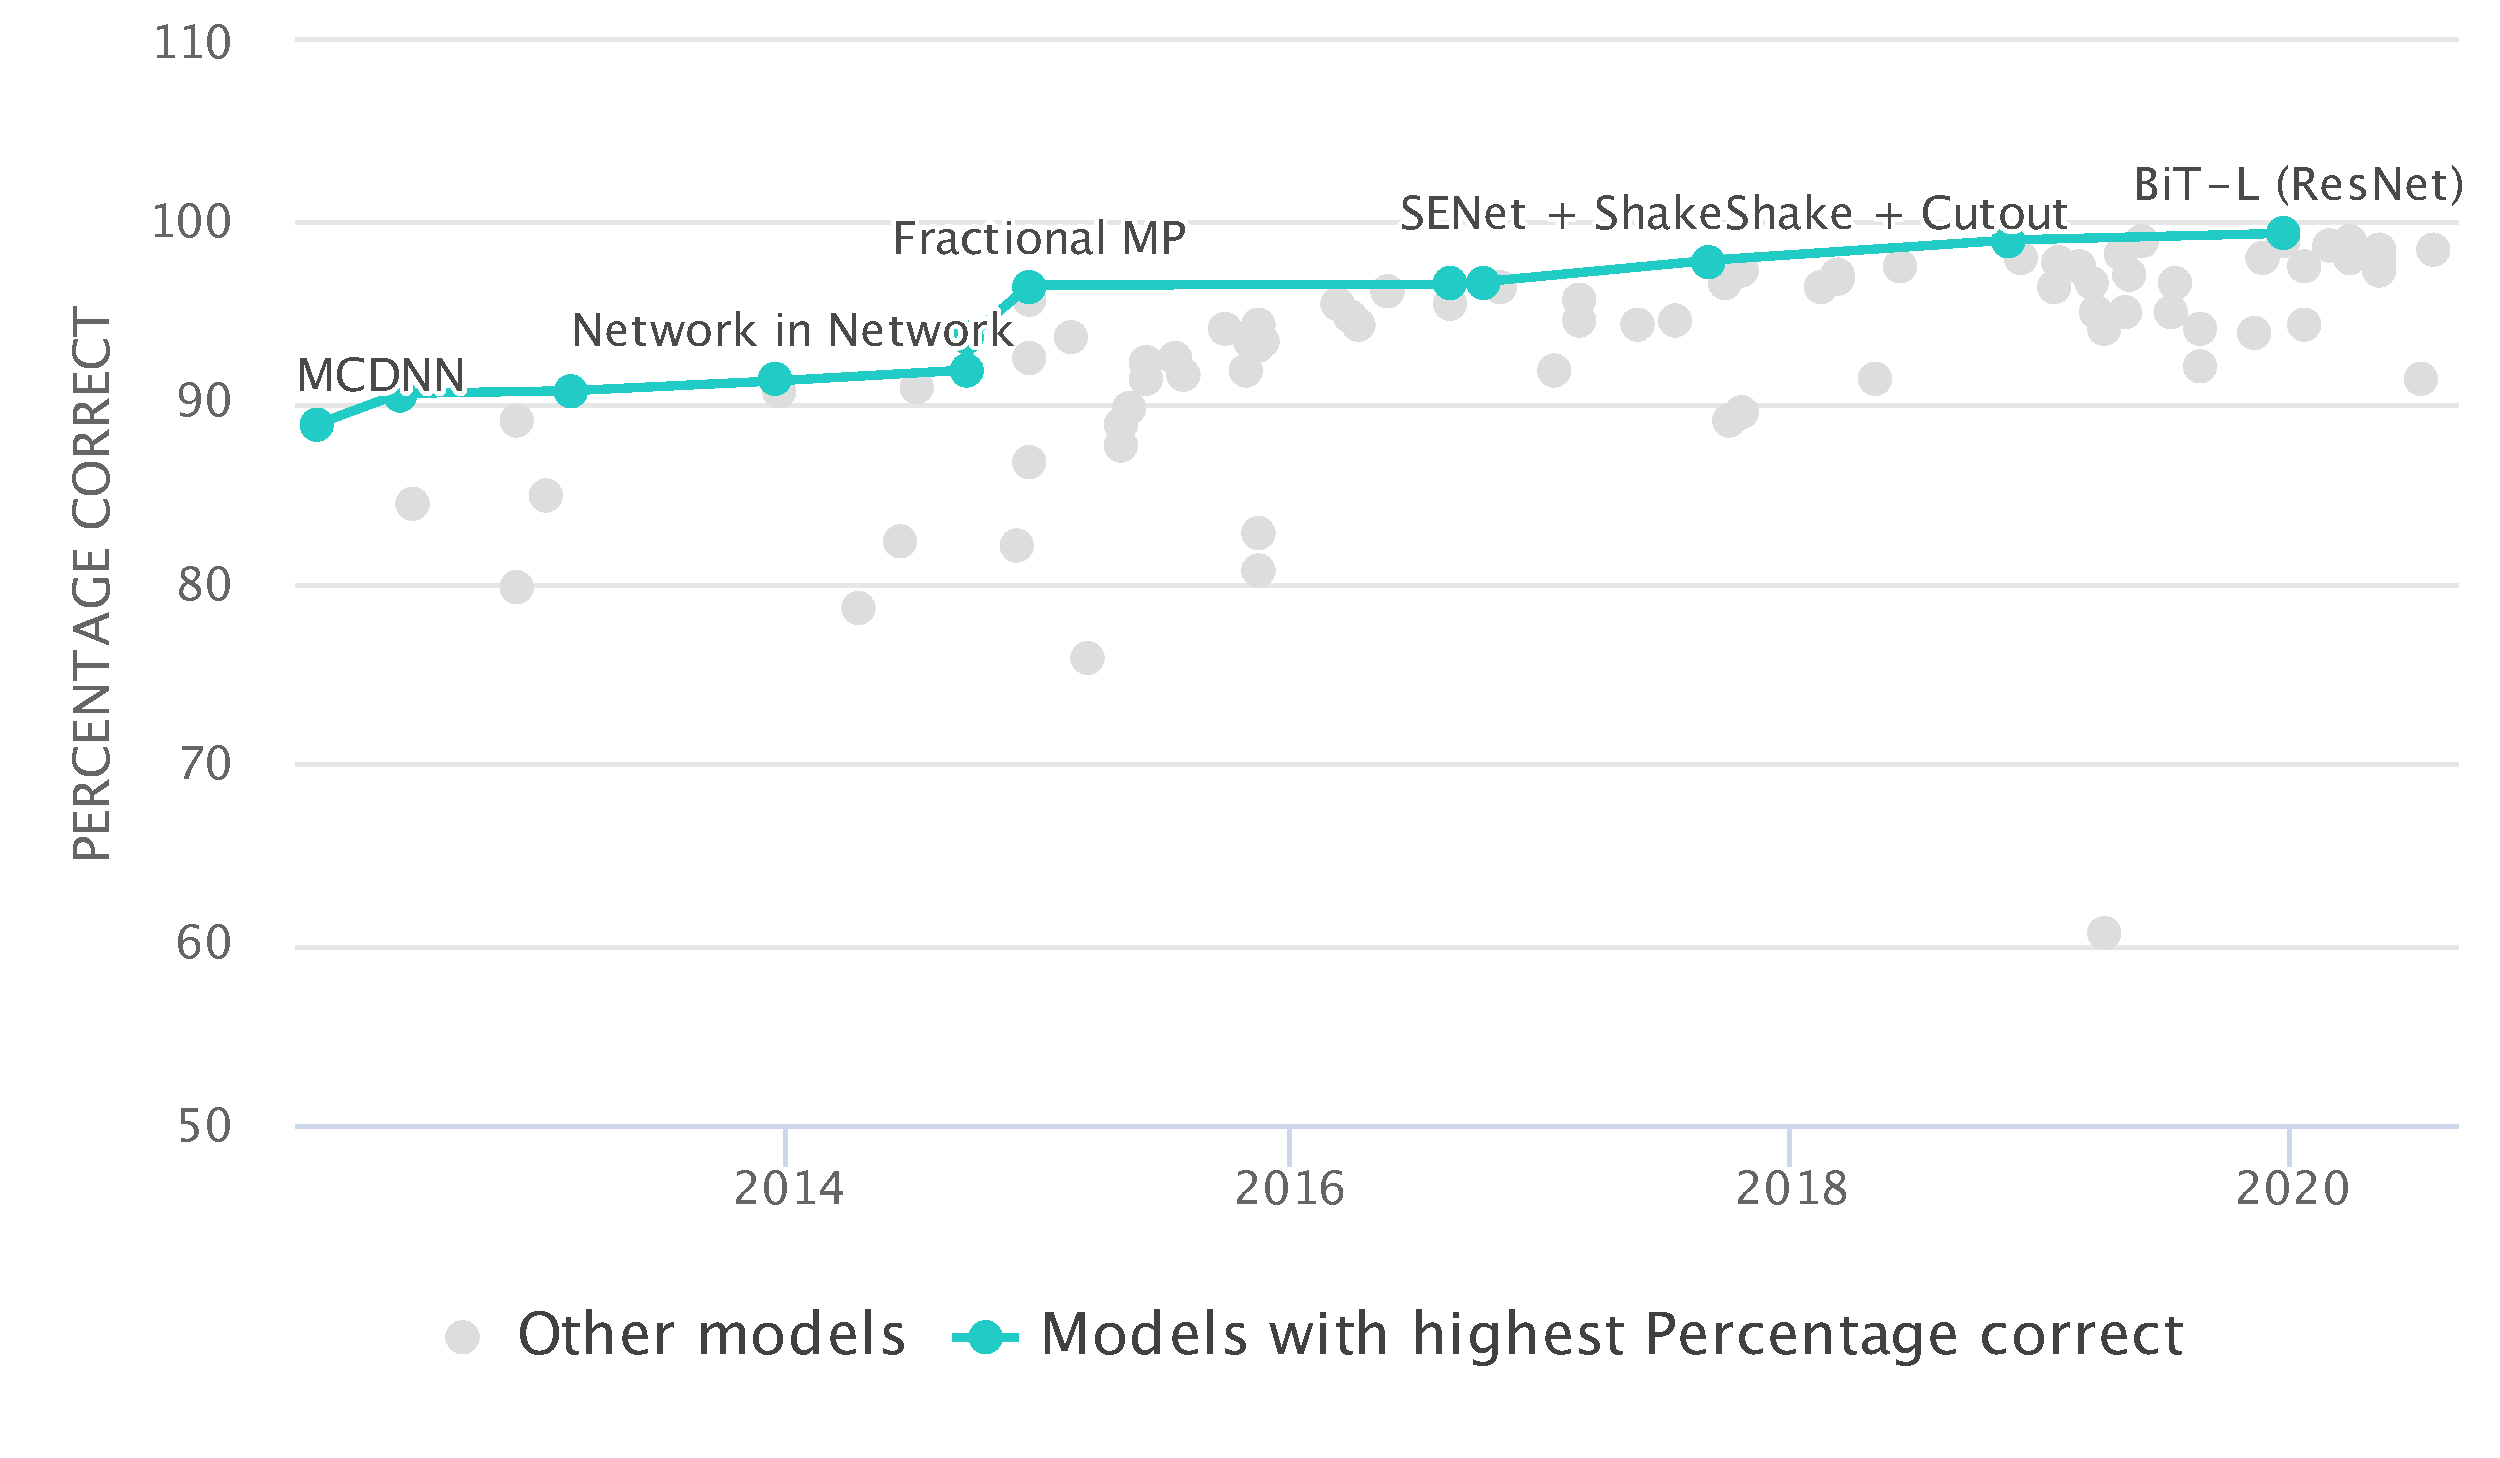
\includegraphics[width=\linewidth]{figures/Cifar10}
        \end{figure} 

        \source{https://paperswithcode.com/sota/image-classification-on-cifar-10}
    \end{frame}

    \begin{frame}{Motivation: Trends on CIFAR-100} 
        \begin{center}
            \Large Test Accuracy: \textbf{CIFAR-100}
        \end{center}

        \begin{figure}[]
            \centering
            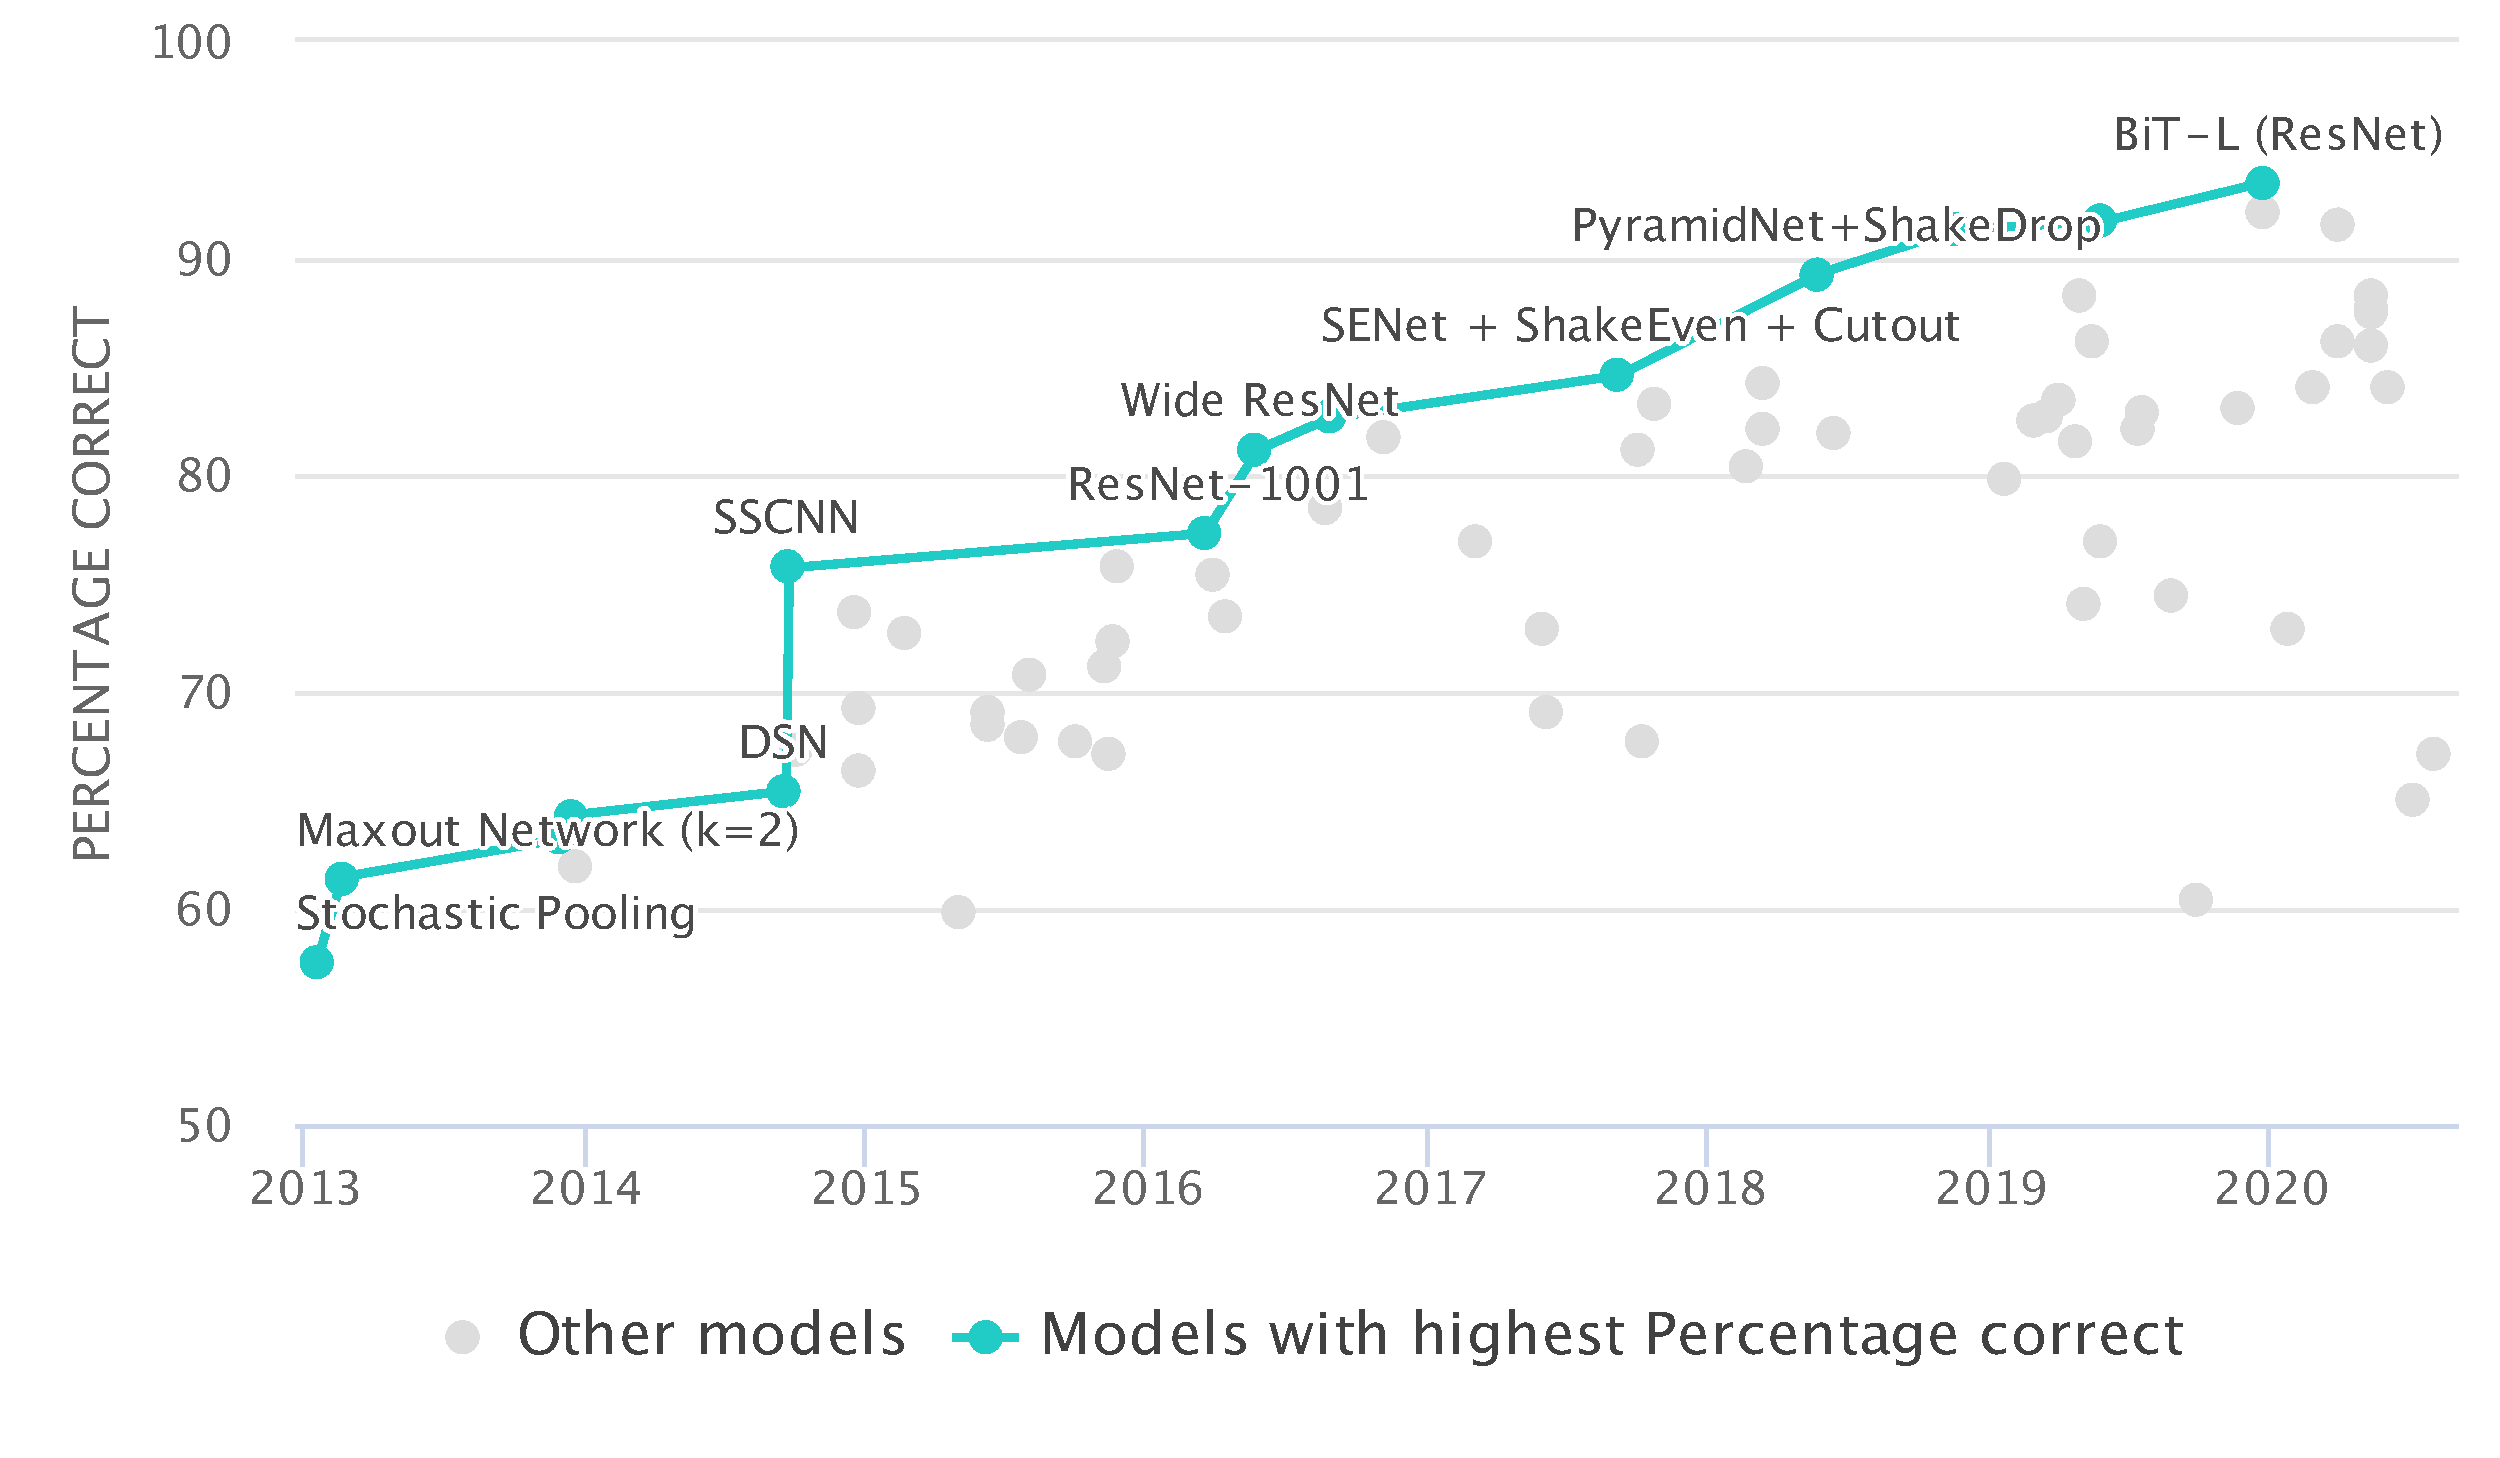
\includegraphics[width=\linewidth]{figures/Cifar100}
        \end{figure} 

        \source{https://paperswithcode.com/sota/image-classification-on-cifar-100}
    \end{frame}

    \begin{frame}{Motivation: Trends on ImageNet} 
        \begin{center}
            \Large Test Accuracy: \textbf{ImageNet}
        \end{center}

        \begin{figure}[]
            \centering
            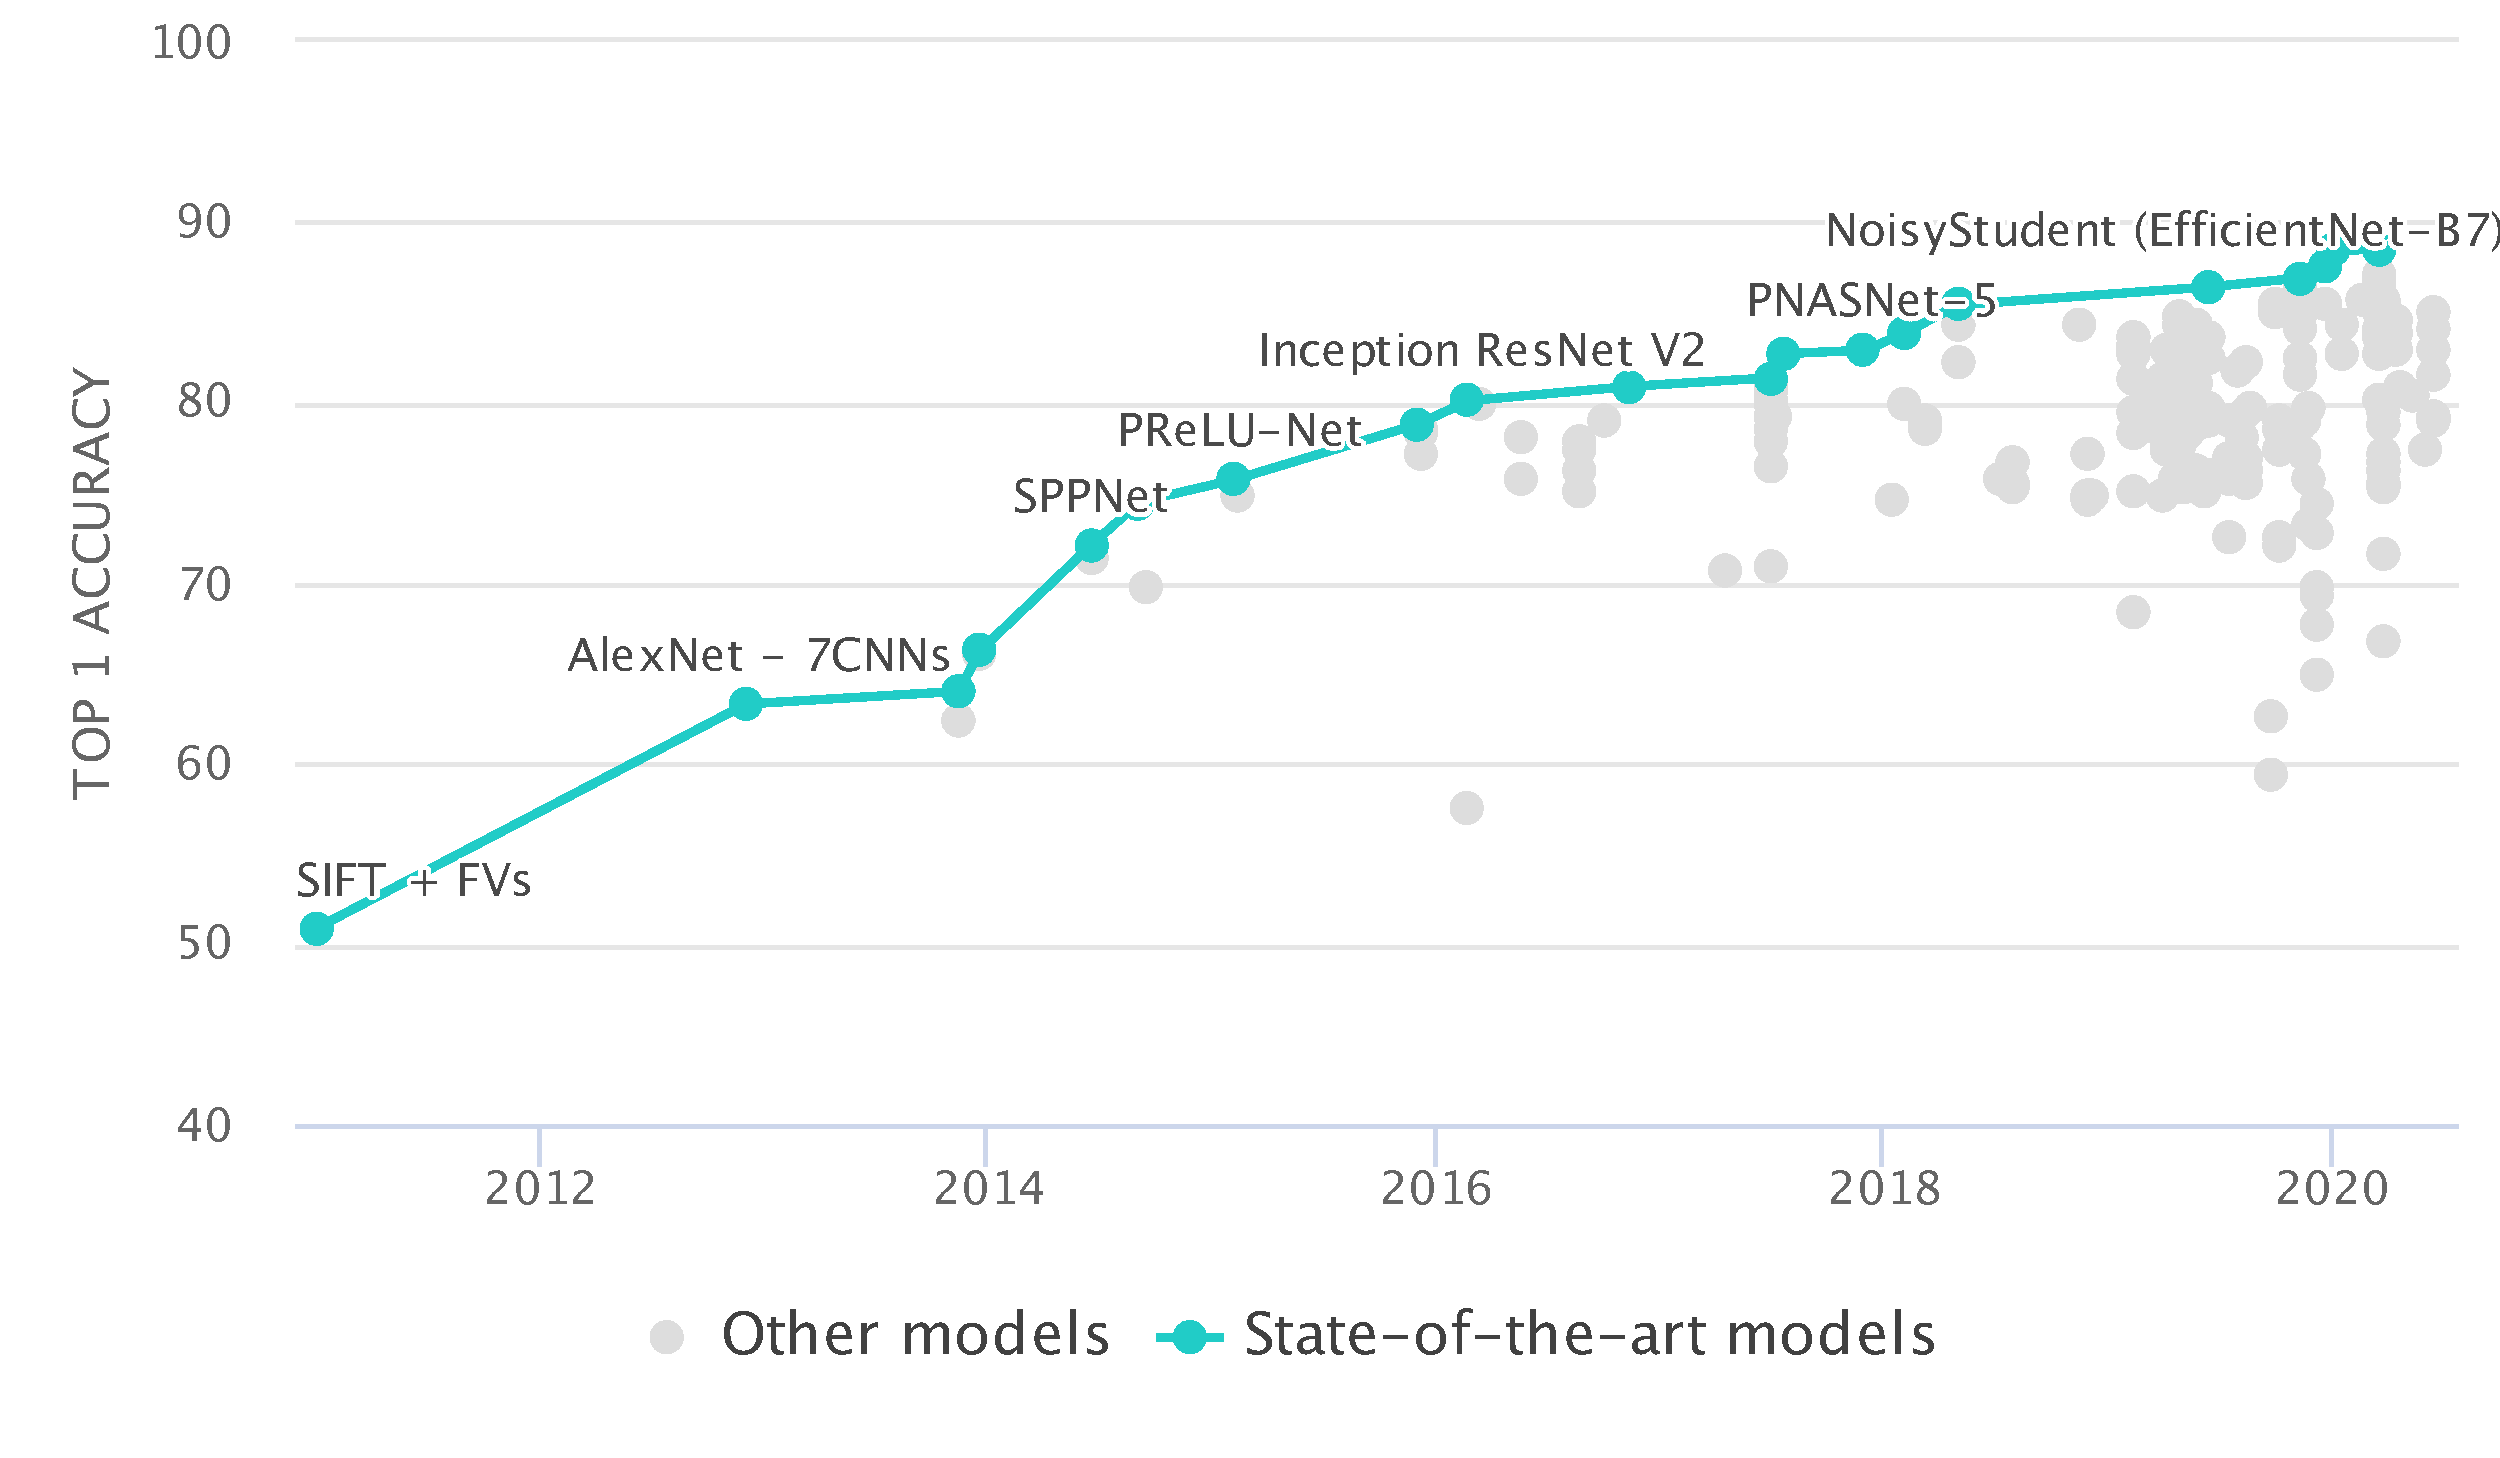
\includegraphics[width=\linewidth]{figures/ImageNet}
        \end{figure} 

        \source{https://paperswithcode.com/sota/image-classification-on-imagenet}
    \end{frame}

    \begin{frame}{Motivation: Better Optimization via Better Models}

        \begin{figure}
            \centering
            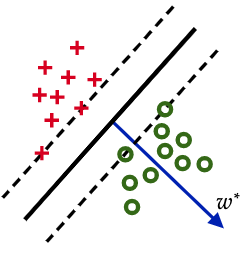
\includegraphics[width=0.38\textwidth]{figures/separable}
            \hspace{0.2em}
            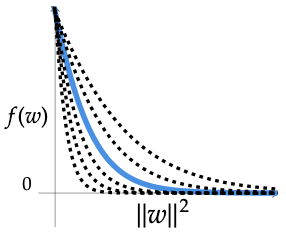
\includegraphics[width=0.45\textwidth]{figures/loss_fn}
        \end{figure}
        \vspace{0.2em}

        \begin{center}
            \large \textbf{Idea}: exploit ``over-parameterization'' for better optimization.\vspace{0.25em}
        \end{center}

    \end{frame}

    \setbeamercolor{background canvas}{bg=lightcyan}

    %% interpolation

    \begin{frame}
       \begin{center}
          \huge Part 1: Interpolation 
       \end{center} 
    \end{frame}

    \setbeamercolor{background canvas}{bg=white}

    \begin{frame}{Interpolation: Assumptions}
        \begin{center}
            \Large 
            \textbf{Goal}: Minimize \( f : \R^d \into \R\), where 
        \end{center}
       
        \vspace{3ex}
        
        \begin{itemize}
            \item \( f \) is \textbf{lower-bounded}: \( \exists \, \wopt \in \R^d \) such that
                \begin{align*}
                    f(\wopt) &\leq f(w) \hspace{1.7em} \tag*{\(\forall \w \in \R^d \), } 
                \end{align*}

            \item \( f \) is L-\textbf{smooth}: \( \w \mapsto \grad(\w) \) is \( L \)-Lipschitz, 
                \begin{align*}
                    \norm{\grad(\w) - \grad(u)}_2 &\leq L \norm{\w - u}_2 \tag*{\(\forall \w, u \in \R^d \),} 
                \end{align*}

            \item (Optional) \( f \) is \( \mu \)-\textbf{strongly-convex}: \( \exists \, \mu \geq 0 \) such that, 
                \begin{align*}
                   f(u) \geq f(\w) + \abr{\grad(\w), u - \w} + \frac{\mu}{2} \norm{u - \w}^2_2 \tag*{\( \forall \w, u \in \R^d \).}
                \end{align*}
        \end{itemize}
     
    \end{frame}

    \begin{frame}{Interpolation: Stochastic First-Order Oracles}

        \textbf{Classic}:
        \begin{enumerate}
            \item At each iteration \( k \), query oracle \oracle{} for stochastic estimates 
                \[ f(\wk, \zk) \quad \text{and} \quad \grad(\wk, \zk). \] 
            \item \( f(\wk, \cdot) \) is a deterministic function of random variable \( \zk \). 
                \vspace{1ex}
            \item \textcolor{red}{\oracle{} is \textbf{unbiased}}, meaning 
            \[ \Ek\sbr{f(\wk, \zk)} = f(\wk) \quad \text{and} \quad \Ek\sbr{\grad(\wk, \zk)} = \grad(\wk). \]% 
        \end{enumerate}%
        \pause%
        \textbf{New}:
        \begin{enumerate}
            \item \textcolor{blue}{\oracle{} is \textbf{individually-smooth}}, meaning \( f(\cdot, \zk) \) is \( \Lmax \)-smooth, 
                \begin{align*}
                    \norm{\grad(\w, \zk) - \grad(u, \zk)}_2 &\leq \Lmax \norm{\w - u}_2 \tag*{\(\forall \w, u \in \R^d \),} 
                \end{align*}
                almost surely.
        \end{enumerate}

    \begin{textblock}{2.5}(0.3,11)
        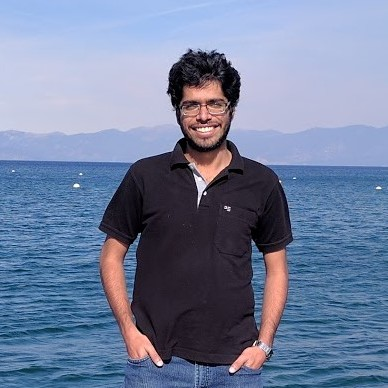
\includegraphics[width=0.4\textwidth]{collaborators/sharan}<2->

        \vspace{0.5ex}

        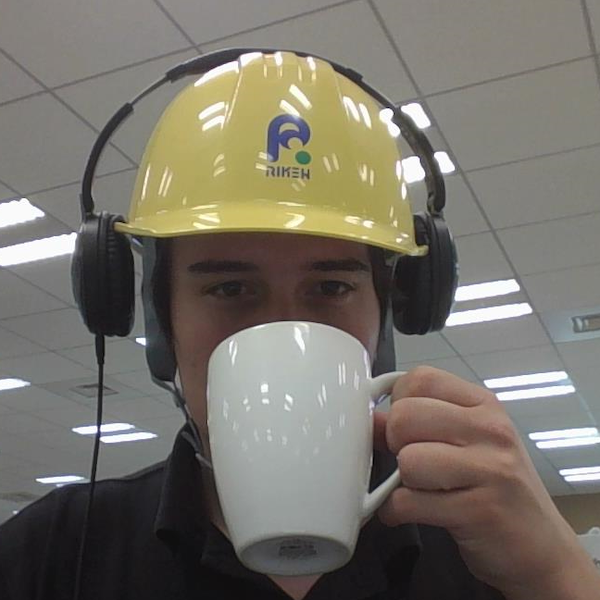
\includegraphics[width=0.4\textwidth]{collaborators/fred}<2->
    \end{textblock}

    \end{frame}

    \begin{frame}{Interpolation: SFOs and Least Squares}
        \vspace{-1ex}

        \[ \textbf{Least Squares}: \wopt \in \argmin \frac{1}{2n} \sum_{i=1}^n \rbr{\abr{w, x_i} - y_i}^2. \]
        
        \vspace{2ex} 
        
        The \textbf{sub-sampling} oracle sets \( \zk \sim \text{Uniform}(1, \ldots, n) \) and returns 
        \[ f(\w, \zk) =  \half \rbr{\abr{w, x_i} - y_i}^2 \quad \text{and} \quad \grad(\wk, \zk) = \rbr{\abr{\w, x_i} - y_i} x_i. \]

        \pause 
        \rule{\textwidth}{0.4pt}
        Observations: 
        \begin{itemize}
            \item \textcolor{red}{\oracle{} is \textbf{unbiased}.} 
            \item \textcolor{blue}{\oracle{} is \( \Lmax = \max_{i} \norm{x_i}^2_2 \) \textbf{individually-smooth}} since 
                    \[ f_{i}(\w) = \half \rbr{\abr{w, x_{i}} - y_{i}}^2, \]
                    is \( \norm{x_{i}}_2^2 \)-smooth for each \( i \in [n] \).
        \end{itemize}

    \end{frame}

    \begin{frame}{Interpolation: Defining Interpolation}
        
        \begin{restatable}[Interpolation: Minimizers]{definition}{interpolationMinima}\label{def:interpolation-minima}
            The pair \( (f, \oracle{}) \) satisfies minimizer interpolation if for all \( \z \in \calZ \),
            \[ f(\w') \leq f(\w) \; \forall \w \in \R^d \implies f(\w', \z) \leq f(\w, \z) \; \forall \w \in \R^d.  \]
        \end{restatable}
        \pause
        \begin{restatable}[Interpolation: Stationary Points]{definition}{interpolationGradients}\label{def:interpolation-gradients}
            The pair \( (f, \oracle{}) \) satisfies stationary-point interpolation if for all \( \z \in \calZ \),
            \[ \grad(\w') = 0 \implies \grad(\w', \z) = 0. \]
        \end{restatable}
        \pause
        \begin{restatable}[Interpolation: Mixed]{definition}{interpolationMixed}\label{def:interpolation-mixed}
            The pair \( (f, \oracle{}) \) satisfies mixed interpolation if for all \( \z \in \calZ \),
            \[ f(\w') \leq f(\w) \; \forall \w \in \R^d \implies \grad(\w', \z) = 0. \]
        \end{restatable}

    \end{frame}

    \begin{frame}{Interpolation: Minimizer}
        \begin{figure}
            \centering 
            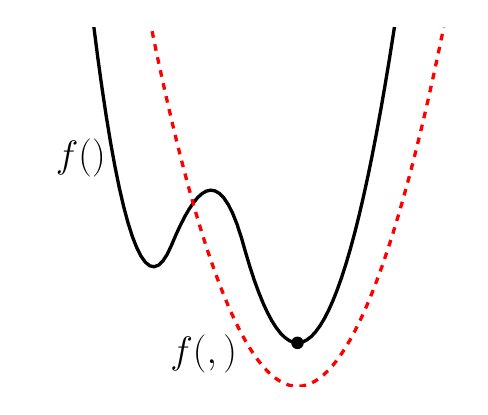
\begin{tikzpicture}[scale=0.8, 
      declare function={
        objective(\x)=      (\x<=-1) * (2*\x*\x + 6*\x + 4)    +
        and(\x>-1, \x<=1) * (\x + 5 - pow(\x,3) - 5*\x*\x) / 4 +
                            (\x>1) * (\x*\x - 5*\x + 4); 
        oracle1(\x)=         (pow(\x - 2.5, 2) / 2 - 3.25);
      }
    ]
    \begin{axis}[
      axis x line=none, axis y line=none,
      ymin=-3.25, ymax=5, ytick={-5,...,5}, ylabel=$y$,
      xmin=-5, xmax=7, xtick={-5,...,7}, xlabel=$x$,
    ]
    \addplot[domain=-5:7, samples=100, objective]{objective(x)};
    \addplot[domain=-5:7, samples=100, oracle]{oracle1(x)};
    
    %% point labels
    \node[label={90:$\wopt$},circle,fill,inner sep=2pt] at (axis cs:2.5,-2.25) {};
    %% function labels
    \node[label={180:$f(\w)$}] at (axis cs:-2.4,2) {};
    \node[label={180:$f(\w, \z)$}] at (axis cs:1.25,-2.5) {};
    \end{axis}
\end{tikzpicture}%
 
        \end{figure}
        
        \interpolationMinima*

    \end{frame}


    \begin{frame}{Interpolation: Stationary-Point}
        \begin{figure}
           \centering 
            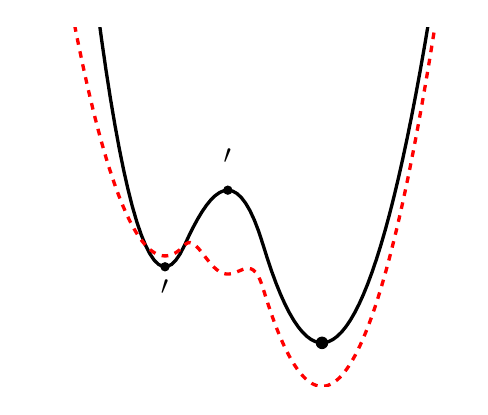
\begin{tikzpicture}[scale=0.8,
      declare function={
        objective(\x)=      (\x<=-1) * (2*\x*\x + 6*\x + 4)    +
        and(\x>-1, \x<=1) * (\x + 5 - pow(\x,3) - 5*\x*\x) / 4 +
                            (\x>1) * (\x*\x - 5*\x + 4); 
        oracle1(\x)=        (\x<=-1) * (pow(x + 1.5, 2))   +
        and(\x>-1, \x<=1) * (-305*pow(\x, 4)/264- 1*pow(\x, 3)/4 + 173*pow(\x,2)/132 - 1*\x/4 - 107/264) +
                            (\x>1) * (pow(x - 2.5, 2) - 3) - 0.25; 
      }
    ]
    \begin{axis}[
      axis x line=none, axis y line=none,
      ymin=-3.25, ymax=5, ytick={-5,...,5}, ylabel=$y$,
      xmin=-5, xmax=6, xtick={-5,...,6}, xlabel=$x$,
    ]
    \addplot[domain=-5:6, samples=100, objective]{objective(x)};
    \addplot[domain=-5:6, samples=200, oracle]{oracle1(x)};
    
    %% point labels
    \node[label={90:$\wopt$},circle,fill,inner sep=2pt] at (axis cs:2.5,-2.25) {};
    \node[label={90:$\w'$},circle,fill,inner sep=1.5pt] at (axis cs:0.1,1.262) {};
    \node[label={270:$\w'$},circle,fill,inner sep=1.5pt] at (axis cs:-1.5,-0.5) {};
    %% function labels
    %\node[label={0:$f(\w)$}] at (axis cs:-2.6,2.5) {};
    %\node[label={180:$f(\w, \z)$}] at (axis cs:1.25,-2.5) {};
    %% plot label
    \end{axis}
\end{tikzpicture}


 
        \end{figure}
        
        \interpolationGradients*

    \end{frame}

    \begin{frame}{Interpolation: Mixed}
        \begin{figure}
           \centering 
            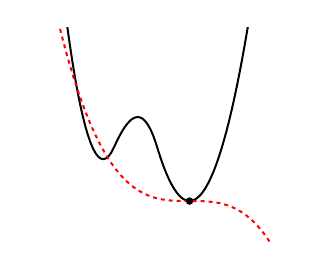
\begin{tikzpicture}[scale=0.48,
      declare function={
        objective(\x)=      (\x<=-1) * (2*\x*\x + 6*\x + 4)    +
        and(\x>-1, \x<=1) * (\x + 5 - pow(\x,3) - 5*\x*\x) / 4 +
                            (\x>1) * (\x*\x - 5*\x + 4); 
        oracle1(\x)=        -(1/30)*pow(x-2.5,3) - 2.25; 
      }
    ]
    \begin{axis}[
      axis x line=none, axis y line=none,
      ymin=-4, ymax=5, ytick={-5,...,5}, ylabel=$y$,
      xmin=-5, xmax=7, xtick={-5,...,7}, xlabel=$x$,
    ]
    \addplot[domain=-5:7, samples=100, objective]{objective(x)};
    \addplot[domain=-5:7, samples=200, oracle]{oracle1(x)};
    
    %% point labels
    \node[label={90:$\wopt$},circle,fill,inner sep=2pt] at (axis cs:2.5,-2.25) {};
    %% function labels
    %\node[label={0:$f(\w)$}] at (axis cs:-2.6,2.5) {};
    %\node[label={180:$f(\w, \z)$}] at (axis cs:1.25,-2.5) {};
    %% plot label
    \end{axis}
\end{tikzpicture}
 
        \end{figure}

        \interpolationMixed*

    \end{frame}

    \begin{frame}{Interpolation: Relationships}

        \begin{restatable}[Interpolation Relationships]{lemma}{interpRelationships}
            Let \( \rbr{f, \oracle{}} \) be arbitrary. 
            Then only the following relationships hold: 
            \begin{align*}
                \text{Minimizer Interpolation} &\implies \text{Mixed Interpolation} \\
                                                                                       & \text{and} &\\
                \text{Stationary-Point Interpolation} &\implies \text{Mixed Interpolation}.
            \end{align*}
            However, if \( f \) and \( f(\cdot, \zk) \) are invex (almost surely) for all \( k \), then the three definitions are equivalent. 
        \end{restatable}
        
    \end{frame}
  
    %% growth conditions

    \setbeamercolor{background canvas}{bg=lightcyan}

    \begin{frame}
       \begin{center}
          \huge Pause 
       \end{center} 
    \end{frame}


    \begin{frame}
       \begin{center}
          \huge Part 2: Growth Conditions 
       \end{center} 
    \end{frame}

    \setbeamercolor{background canvas}{bg=white}
    
    \begin{frame}{Growth Conditions: Iteration Complexity}
        \Large 
        
        \textbf{Question}: for how many iterations do we need to run SGD to obain 
        \[ \E\sbr{f(\wk) - f(\wopt)} \leq \epsilon \] 
        if minimizer interpolation holds?

       \vspace{4ex}
       \pause 
       \textbf{Two Approaches}: 
       \begin{enumerate}
           \item Use interpolation in a direct analysis of SGD. 
           \item Relate interpolation to ``nice'' properties of \( \oracle{} \). 
       \end{enumerate}

    \end{frame}

    \begin{frame}{Growth Conditions: Well-behaved Oracles}
        
        \mbox{\large There are many possible regularity assumptions on \oracle{}.} 

        \begin{align*} 
            \textbf{Bounded Gradients}:& \quad  \E\sbr{\norm{\grad(\w, \zk)}} \leq \textcolor{red}{\sigma^2}, \\ 
           \intertext{\hspace{3.5em} \small\textbullet{} Proposed by Robbins and Monro in their analysis of SGD. }
           \textbf{Bounded Variance}:& \quad \E \sbr{\norm{\grad(\w, \zk)}^2} \leq \textcolor{blue}{\norm{\grad(\w)}^2} + \textcolor{red}{\sigma^2}, \\
           \intertext{\hspace{3.5em} \small \textbullet{} Commonly used in the stochastic approximation setting.}
           \textbf{Strong Growth+Noise}:& \quad  \E \sbr{\norm{\grad(\w, \zk)}} \leq \rho \, \textcolor{blue}{\norm{\grad(\w)}^2} + \textcolor{red}{\sigma^2}.
           \intertext{\hspace{3.5em} \small \textbullet{} Satisfied when \oracle{} is individually-smooth. }
       \end{align*} 

    \end{frame}

    \begin{frame}{Growth Conditions: Strong and Weak Growth}

        \mbox{\large We obtain the strong and weak growth conditions as follows: } 

        \begin{align*} 
            \textbf{Strong Growth+Noise}:& \quad  \E \sbr{\norm{\grad(\w, \zk)}} \leq \rho \, \textcolor{blue}{\norm{\grad(\w)}^2} + \textcolor{red}{\sigma^2}. \\
           \intertext{\hspace{3.5em} \small \textbullet{} Does not imply interpolation. }
           \pause
            \textbf{Strong Growth}:& \quad  \E \sbr{\norm{\grad(\w, \zk)}} \leq \rho \, \textcolor{blue}{\norm{\grad(\w)}^2}.\\
            \intertext{\hspace{3.5em} \small \textbullet{} Implies \textbf{stationary-point} interpolation. }
           \pause
            \textbf{Weak Growth}:& \quad  \E \sbr{\norm{\grad(\w, \zk)}} \leq \alpha \, \textcolor{purple}{\rbr{f(\w) - f(\wopt)}}. 
            \intertext{\hspace{3.5em} \small \textbullet{} Implies \textbf{mixed} interpolation. }
       \end{align*} 

    \begin{textblock}{2.5}(0.3,7)
        \centering
        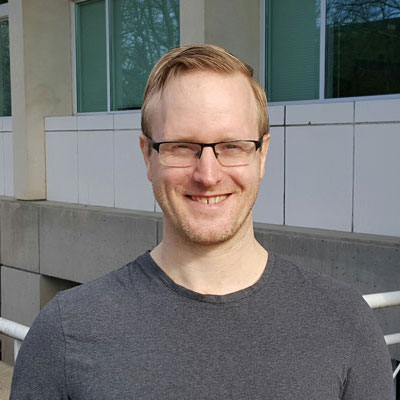
\includegraphics[width=0.4\textwidth]{collaborators/mark}<2->
        
\includegraphics[width=0.4\textwidth]{collaborators/nicolas}<2->
    \end{textblock}

    \begin{textblock}{2.5}(0.3,10)
        \centering
        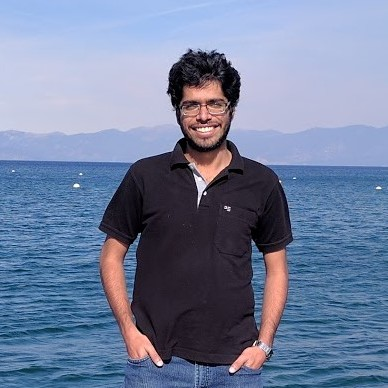
\includegraphics[width=0.4\textwidth]{collaborators/sharan}<3->
        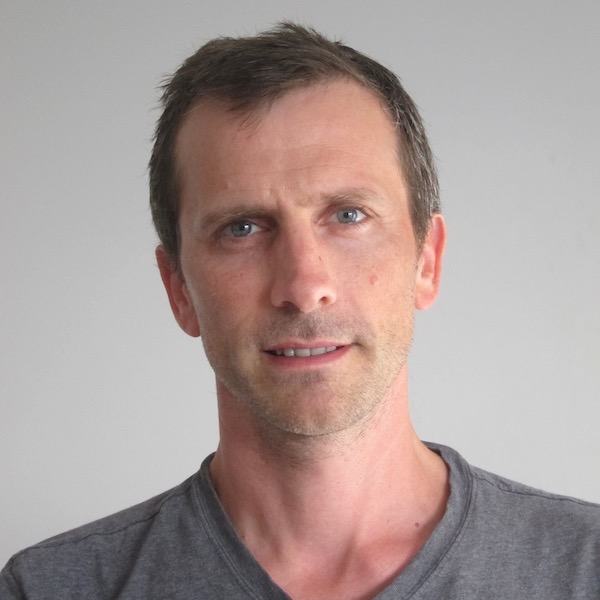
\includegraphics[width=0.4\textwidth]{collaborators/francis}<3->

        \vspace{0.5ex}

        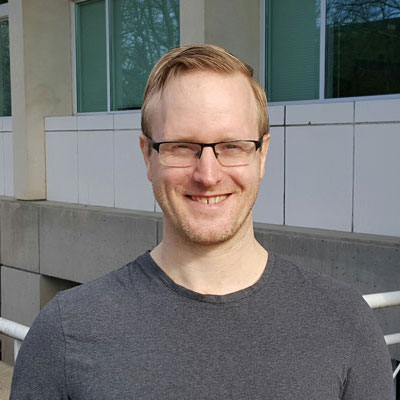
\includegraphics[width=0.4\textwidth]{collaborators/mark}<3->
    \end{textblock}


    \end{frame}

    \begin{frame}{Growth Conditions: Interpolation + Smoothness}
    \begin{center}
            
        \vspace{-2ex}
        \begin{minipage}[t]{0.82\textwidth}
            \vspace{-1.45ex}
            \begin{restatable}[Interpolation and Weak Growth]{lemma}{interpToWGC}~\label{lemma:interpolation-to-wgc}
                Assume \( f \) is \( L \)-smooth and \oracle{} is \( \Lmax \) individually- smooth. 
                If minimizer interpolation holds, then weak growth also holds with
                \[ \wgc \leq \frac{L_{\text{max}}}{L}. \]
            \end{restatable}
           

            \begin{restatable}[Interpolation and Strong Growth]{lemma}{interpToSGC}~\label{lemma:interpolation-to-sgc}
                Assume \( f \) is \( L \)-smooth and \( \mu \) strongly-convex and \oracle{} is \( \Lmax \) individually-smooth. 
                If minimizer interpolation holds, then strong growth also holds with 
                \[ \rho \leq \frac{L_{\text{max}}}{\mu}. \]
            \end{restatable}
        \end{minipage}
        \begin{minipage}[t]{0.15\textwidth}
            \begin{figure}[t]
                \centering
                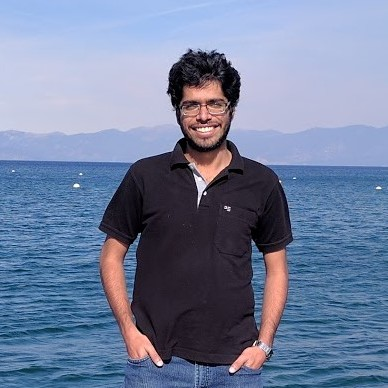
\includegraphics[width=0.8\textwidth]{collaborators/sharan}

                \vspace{0.5ex}

                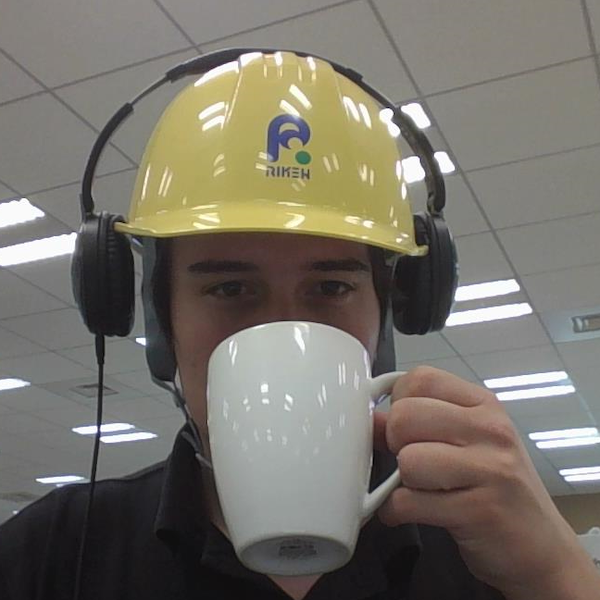
\includegraphics[width=0.8\textwidth]{collaborators/fred}
            \end{figure} 
        \end{minipage}
        
    \end{center}
    \end{frame}

    \setbeamercolor{background canvas}{bg=lightcyan}

    %% stochastic gradient descent (sgd) 
    
    \begin{frame}
       \begin{center}
          \huge Part 3: Stochastic Gradient Descent 
       \end{center} 
    \end{frame}
    
    \setbeamercolor{background canvas}{bg=white}

    \begin{frame}{SGD}
       
    \end{frame}

    \begin{frame}{Line Search}
       SGD 
    \end{frame}

    \begin{frame}{Acceleration}
       SGD 
    \end{frame}

    %% end slide
    \setbeamercolor{background canvas}{bg=lightcyan}

    \begin{frame}{}
        \begin{center}
        \huge Thanks for Listening!
        \end{center}
    \end{frame}

    \setbeamercolor{background canvas}{bg=white}


    \begin{frame}{Acknowledgements}
     
        \begin{figure}
            \centering
            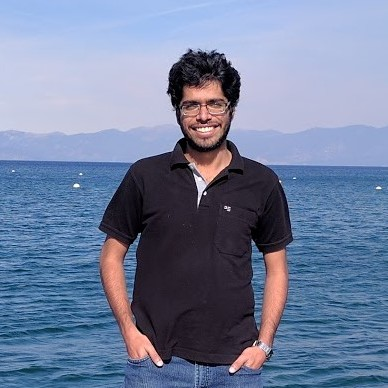
\includegraphics[width=0.18\textwidth]{collaborators/sharan}
            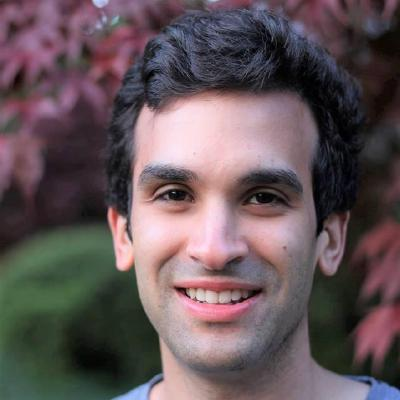
\includegraphics[width=0.18\textwidth]{collaborators/issam}
            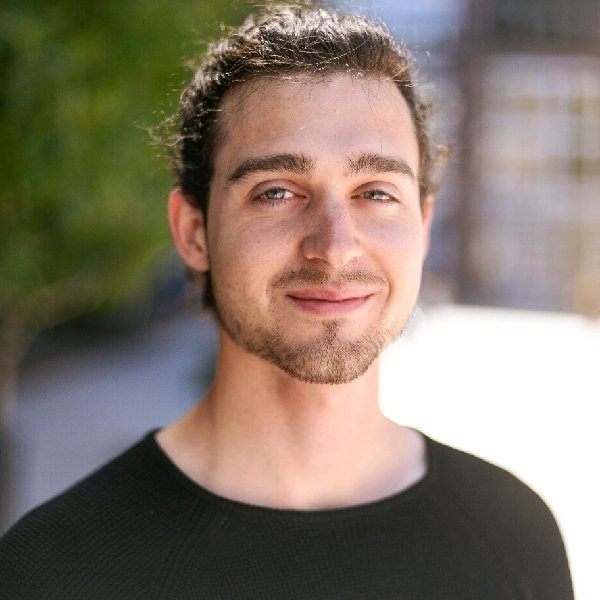
\includegraphics[width=0.18\textwidth]{collaborators/gauthier}
            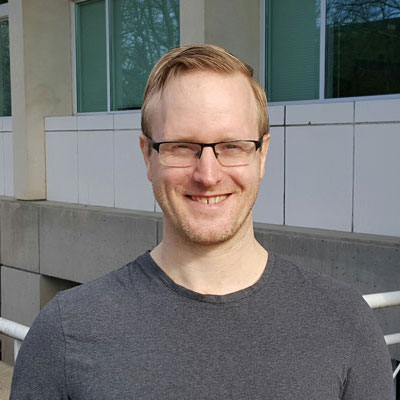
\includegraphics[width=0.18\textwidth]{collaborators/mark}
            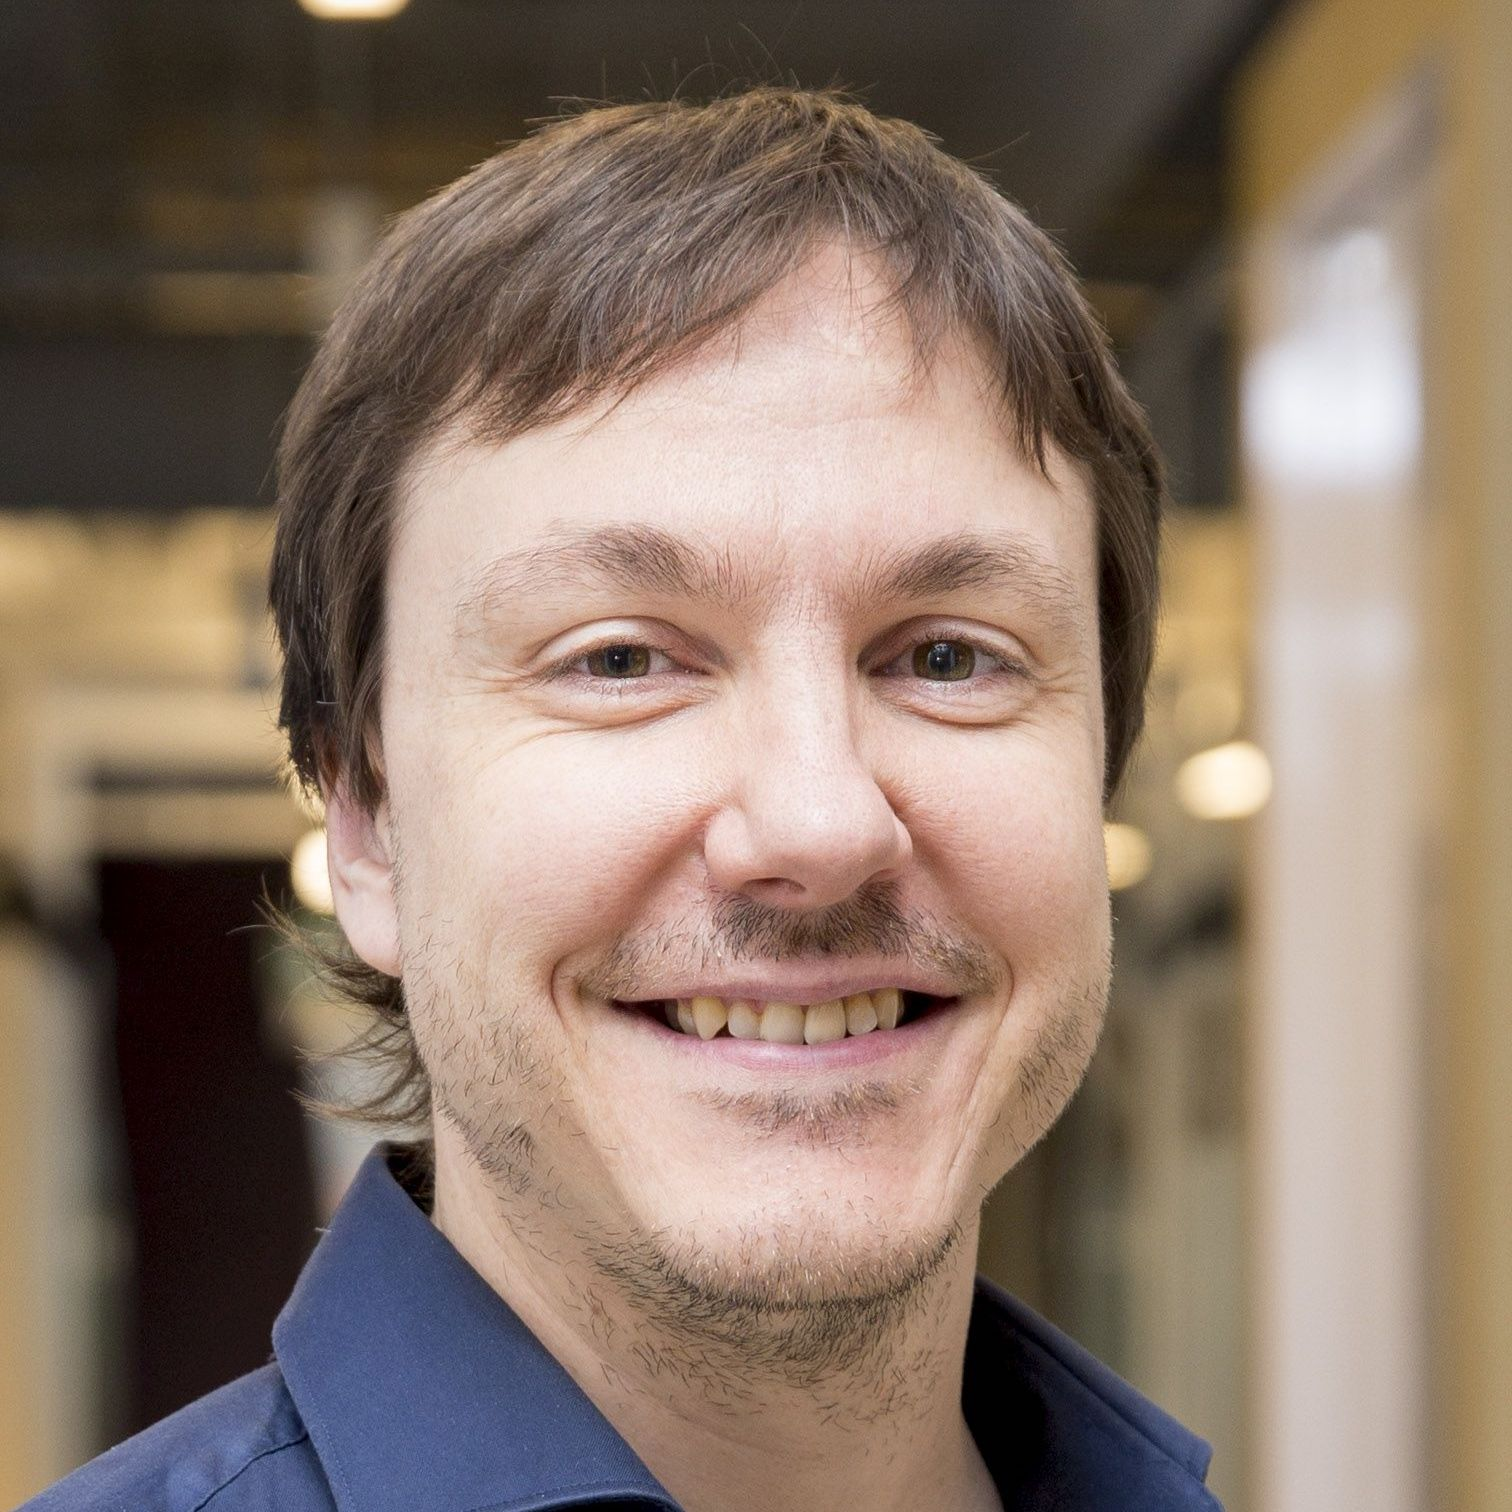
\includegraphics[width=0.18\textwidth]{collaborators/simon}

            \vspace{0.4ex}%

            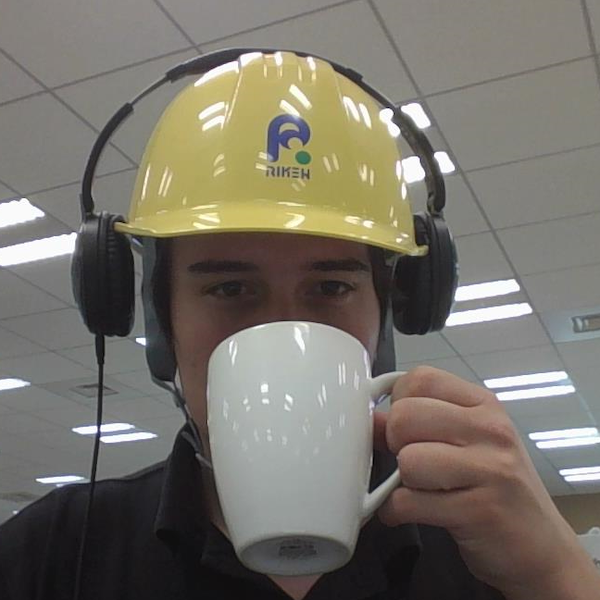
\includegraphics[width=0.18\textwidth]{collaborators/fred}
            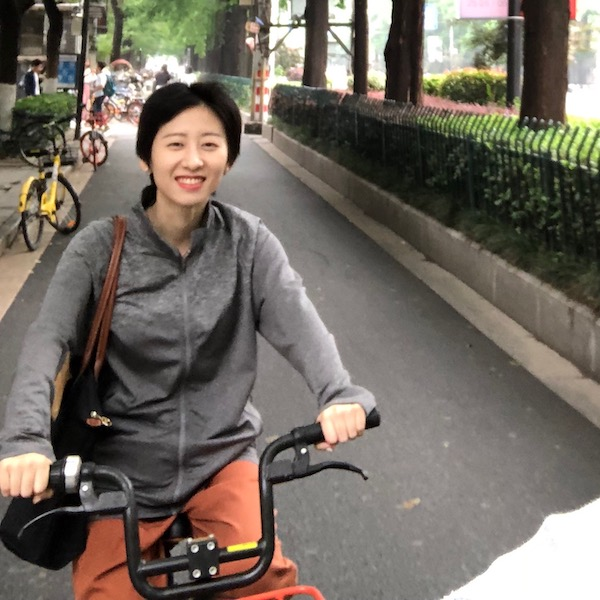
\includegraphics[width=0.18\textwidth]{collaborators/cathy}
            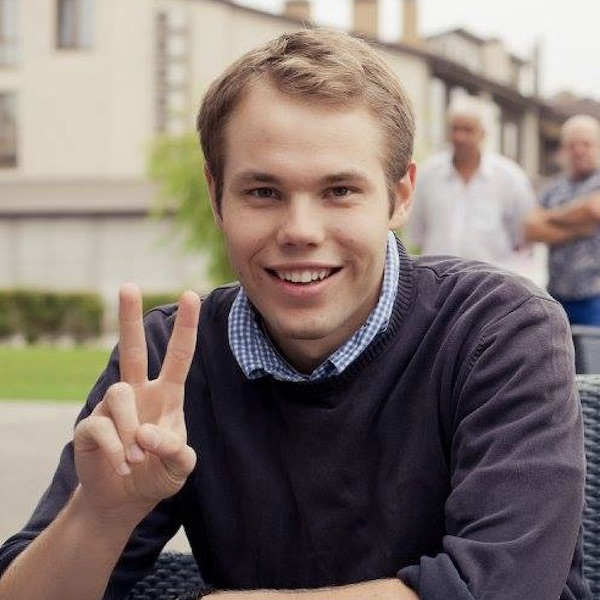
\includegraphics[width=0.18\textwidth]{collaborators/wilder}
            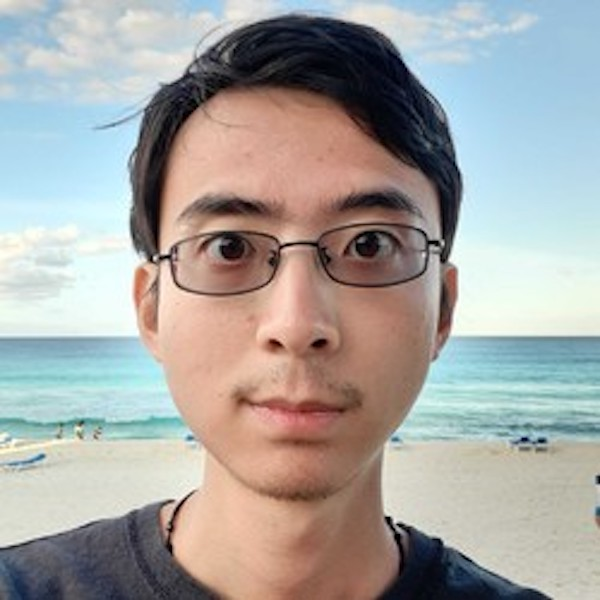
\includegraphics[width=0.18\textwidth]{collaborators/joey}
        \end{figure}

        \textbf{Left to right}:
            \href{https://vaswanis.github.io/}{Sharan Vaswani}, \href{https://issamlaradji.github.io/}{Issam Laradji}, \href{https://gauthiergidel.github.io/}{Gauthier Gidel}, \href{https://www.cs.ubc.ca/~schmidtm/}{Mark Schmidt}, \href{http://www.iro.umontreal.ca/~slacoste/}{Simon Lacoste-Julien}, \href{https://fkunstner.github.io/}{Frederik Kunstner}, \href{https://www.cs.ubc.ca/~mengxixi/}{Si Yi Meng}, \href{https://wilderlavington.github.io/}{Jonathan Lavington}, \href{https://joeyandbluewhale.github.io/}{Yihan Zhou}, and Betty Shea. 
    
        \end{frame}
    %% bibliography
    \begin{frame}[allowframebreaks]{References}
        \bibliographystyle{plainnat}
        \bibliography{refs}
    \end{frame}


\end{document}
